\section{Chọn hệ quản trị và Ánh xạ Kiểu dữ liệu}

Theo quy trình thiết kế cơ sở dữ liệu, thiết kế vật lý không làm thay đổi ý nghĩa dữ liệu mà quyết định cách hệ quản trị lưu trữ, đọc, ghi và tìm kiếm dữ liệu tối ưu nhất dựa trên tải công việc.

\subsection{Chọn hệ quản trị cơ sở dữ liệu}

Hệ thống sử dụng hệ quản trị SQL Server, triển khai qua Docker để mọi thành viên trong nhóm làm việc trên cùng một môi trường.


\begin{lstlisting}[style=sqlstyle]
docker run -e "ACCEPT_EULA=Y" -e "MSSQL_SA_PASSWORD=<mat_khau>" \
  -p 1433:1433 --name sqlserver-tkcsdl \
  -d mcr.microsoft.com/mssql/server:2022-latest
\end{lstlisting}



\begin{figure}[H]
    \centering
        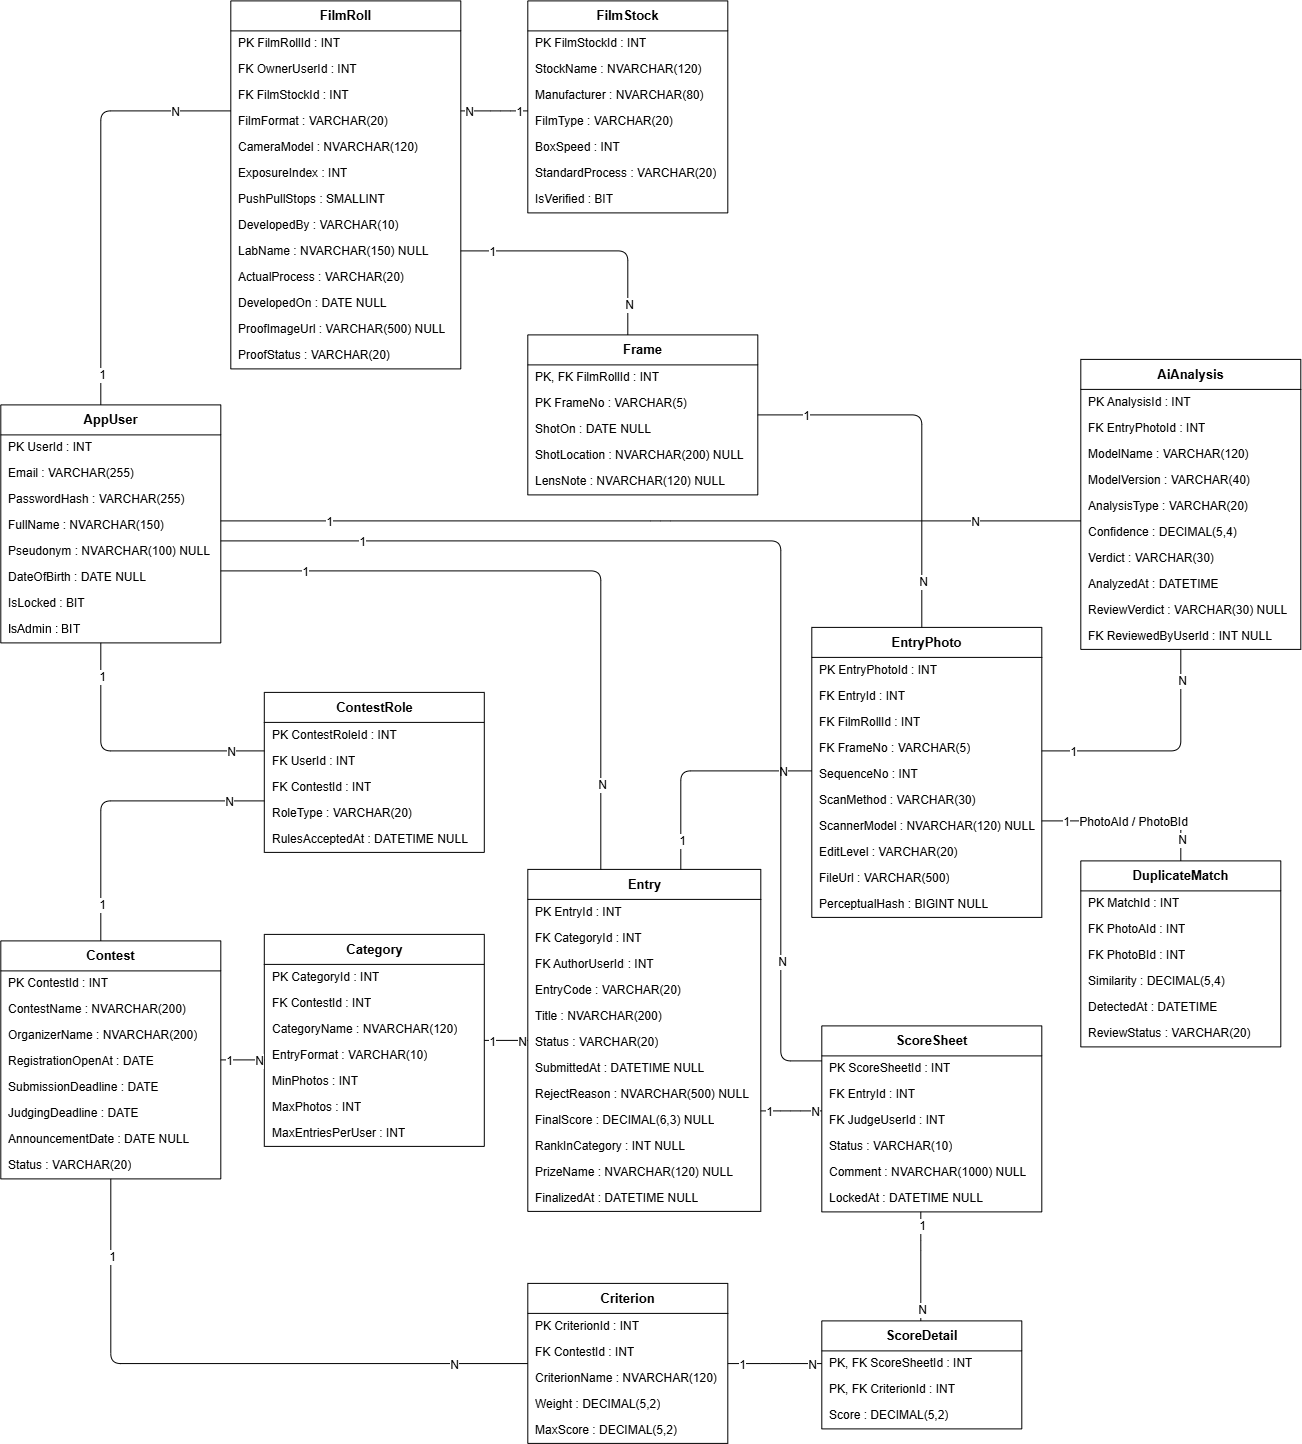
\includegraphics[width=\textwidth]{images/So_do_vat_ly.png}
    \caption{Sơ đồ thiết kế vật lý (Physical Diagram)}
    \label{fig:4.1}
\end{figure}


\subsection{Ánh xạ Kiểu dữ liệu và Ràng buộc}

Đầu vào của thiết kế vật lý gồm lược đồ logic đã đạt BCNF ở Chương 3 cùng tập khóa và ràng buộc. Hệ thống tiến hành ánh xạ sang SQL Server như sau:


\begin{itemize}
    \item \texttt{INT IDENTITY}: dùng cho khóa chính thay thế của các thực thể cốt lõi, cho khóa gọn và chỉ mục hiệu quả hơn chuỗi UUID.
    \item \texttt{NVARCHAR(n)}: dùng cho trường văn bản có ký tự tiếng Việt, ví dụ \texttt{ContestName}, \texttt{Title}, \texttt{FullName}.
    \item \texttt{VARCHAR(n)}: dùng cho trường không dấu, ví dụ \texttt{Email}, \texttt{PasswordHash}, \texttt{EntryCode}.
    \item \texttt{DECIMAL(p,s)}: dùng cho điểm số và trọng số cần độ chính xác tuyệt đối. Không dùng \texttt{FLOAT} vì sai số làm tròn có thể đổi thứ hạng.
    \item \texttt{SMALLINT}: dùng cho \texttt{PushPullStops} vì giá trị nằm trong khoảng hẹp và có thể âm.
    \item \texttt{BIGINT}: dùng cho \texttt{PerceptualHash} vì mã băm cảm nhận là số nguyên 64 bit, vượt quá miền giá trị của \texttt{INT}.
\end{itemize}


Các ràng buộc toàn vẹn gồm \texttt{PRIMARY KEY} để định danh thực thể, \texttt{FOREIGN KEY} để duy trì toàn vẹn tham chiếu, \texttt{NOT NULL} cho trường bắt buộc, \texttt{UNIQUE} cho khóa nghiệp vụ và \texttt{CHECK} cho các ràng buộc miền giá trị nêu ở BR-5. SQL Server không hỗ trợ hành động tham chiếu \texttt{RESTRICT}; các khóa ngoại ghi \texttt{RESTRICT} trong từ điển dữ liệu được hiện thực bằng \texttt{NO ACTION}, mặc định của SQL Server, nên thao tác xóa bản ghi cha bị từ chối khi vẫn còn bản ghi con tham chiếu.

